%-------------------------------------------------------------------------------------------------------------
%       P A R Á M E T R O S   D E   C O M P I L A C I Ó N
%--------------------------------------------------------------
% PDFLaTeX --> BibTeX (x2) --> PDFLaTeX (x2) --> Ver PDF
%--------------------------------------------------------------------------------------------------------------
%                 R E C O M E N D A C I O N E S
%----------------------------------------------------------
% SE RECOMIENDA AMPLIAMENTE NO EDITAR EL DOCUMENTO "example.sty" o "portadaposgradoMCM.sty" QUE CONTIENE LAS CONDICIONES Y ESPECIFICACIONES PROPUESTAS POR EL DEPARTAMENTO
% EL DOCUMENTO "biblio.bib" CONTIENE LA BIBLIOGRAFÍA CON UN PAR DE EJEMPLOS
%--------------------------------------------------------------------------------------------------------------
%                A J U S T E S   D E   I N I C I O 
%--------------------------------------------------------------------------------------------------------------
\PassOptionsToPackage{usenames,dvipsnames}{color}% NO EDITAR 
\documentclass[letterpaper,openright,12pt, oneside, spanish]{book}% NO EDITAR 
\usepackage{example}% NO EDITAR 
\usepackage{portada_oficial_itm}% NO EDITAR
%----------------------------------------------------------
%                D A T O S   P O R T A D A
%----------------------------------------------------------
\author{Br. Giovanny González Baltazar}%EDITAR
\title{Arquitectura para control inteligente de tráfico urbano}%EDITAR
\institucion{instituto tecnológico de mérida}%NO EDITAR
\departamento{división de estudios profesionales}%NO EDITAR
\programa{departamento de sistemas}%EDITAR
\grado{ingeniero(a)}%EDITAR
\asesor{Dr. Joel Antonio Trejo Sánchez}
\coasesor{Dr. Mauricio Gabriel Orozco del Castillo}
%--------------------------------------------------------------------------------------------------------------
%                        D O C U M E N T O
%--------------------------------------------------------------------------------------------------------------
\begin{document}  
%--------------------------------------------------------------------------------------------------------------
%                 C U E R P O   P R E L I M I N A R
%--------------------------------------------------------------------------------------------------------------
\pagenumbering{Roman} % Númeración Romana		
\maketitle % Compila parametros de la portada
\newpage % Nueva página
\afterpage{\blankpage}
%\includepdf[pages=-]{Adjuntos/firmas.pdf} %  Firmas de impresión definitiva
\chapter*{Dedicatoria} % si no queremos que añada la palabra "Capitulo"
\addcontentsline{toc}{chapter}{Dedicatoria} % si queremos que aparezca en el Í­ndice
\markboth{Dedicatoria}{Dedicatoria} % encabezado

\linespread{1.3}
{\Huge{(\textit{Página de dedicatoria})}}
\clearpage % Incluye la dedicatoria
\chapter*{Agradecimientos} % si no queremos que añada la palabra "Capitulo"
\addcontentsline{toc}{chapter}{Agradecimientos} % si queremos que aparezca en el Í­ndice
\markboth{Agradecimientos}{Agradecimientos} % encabezado
\linespread{1.3}
{\Huge{(\textit{Página de agradecimientos})}}
\clearpage % Start a new page % Incluye los agradecimientos
\setcounter{page}{1} % Empieza la numeración Romana
\chapter*{Resumen} % si no queremos que añada la palabra "Capitulo"
\addcontentsline{toc}{chapter}{Resumen} % si queremos que aparezca en el Í­ndice
\markboth{RESUMEN}{RESUMEN} % encabezado
\noindent \rule{0.9\textwidth}{1.0pt} \newline
\noindent \textbf{\textit{Palabras clave}: }\newline
\noindent \rule{0.9\textwidth}{1.0pt}
\ \newline
\par
\linespread{1.3}
{\Huge{(\textit{Página de resumen})}}
\clearpage % Nueva página


% TODO: Como mi trabajo amplía al del Dr. y al del otro chavo, citarlos aquí en la intro % Incluye resumen
\chapter*{Abstract} % si no queremos que añada la palabra "Capitulo"
\addcontentsline{toc}{chapter}{Abstract} % si queremos que aparezca en el Í­ndice
\markboth{ABSTRACT}{ABSTRACT} % encabezado
\noindent \rule{0.9\textwidth}{1.0pt} \newline
\noindent \textbf{\textit{Keywords}:} \newline
\noindent \rule{0.9\textwidth}{1.0pt}
\ \newline
\par
\linespread{1.3}
{\Huge{(\textit{Abstract page})}}
\clearpage % Nueva página
 % Incluye abstract
\newpage
\tableofcontents %  Crea índice
\newpage
\listoftables % Lista de Tablas
\newpage
\listoffigures % Lista de Figuras
\newpage
\chapter*{Nomenclatura} % si no queremos que añada la palabra "Capitulo"
\addcontentsline{toc}{chapter}{Nomenclatura} % si queremos que aparezca en el Í­ndice
\markboth{NOMENCLATURA}{NOMENCLATURA} % encabezado
\linespread{1.3}

\begin{longtable}{p{5mm} c p{120mm} }
	\multicolumn{3}{l}{Glosario}\\
	\\
	A & \qquad\qquad & Área, $m^{2}$.\\
	%$B^{0}$ & \qquad\qquad & Campo magnético, $T$.\\
	c & \qquad\qquad & Velocidad del sonido, $m/s$.\\
	C & \qquad\qquad & Concentración, $m$.\\
	D & \qquad\qquad & Diámetro, $m$.\\
	
	\\
	\multicolumn{3}{l}{Letras griegas}\\
	\\
	$\alpha$ & \qquad\qquad & alpha, $unidad \alpha$. \\	% Editar
	$\beta$ & \qquad\qquad & beta, $unidad \beta$.\\	% Editar
	$\gamma$ & \qquad\qquad & gamma, $unidad \gamma$.\\	% Editar

	
	\\
		\multicolumn{3}{l}{Lista de siglas}\\
	\\
	CAD & \qquad\qquad  & Diseño Asistido por Computadora.\\ % Editar
	GUI	& \qquad\qquad	& Interfaz Gráfica de Usuario.\\
	CFL	& \qquad\qquad	& Condición de Courant-Friedrichs-Lewy.\\
	
\end{longtable}
\clearpage % Incluye nomenclatura
\newpage
%---------------------------------------------------------------------------------------------------------------
%                 C U E R P O   P R I N C I P A L
%---------------------------------------------------------------------------------------------------------------
\pagenumbering{arabic} %Numeración Arábiga
\setcounter{page}{1}
\clearpage
\newpage
\thispagestyle{empty}
\vspace*{\fill}
\begingroup
\centering
\begin{flushright}{\fontsize{50}{60}\selectfont CAPÍTULO 1}\end{flushright}
\vspace{10 mm}
\begin{flushright}{\fontsize{30}{40}\selectfont INTRODUCCIÓN }\end{flushright}
\endgroup
\vspace*{\fill}
\newpage

\chapter{Introducción} % con la palabra capitulo
\graphicspath{{./../imagenes/}}
\linespread{1.3}
\hypertarget{introducciuxf3n}{%
\section{Introducción}\label{introducciuxf3n}}

Los países en vías de desarrollo en innumerables ocasiones han tenido
que afrontar problemas a los que otros países ya se han enfrentado
antes. Las que antes eran pequeñas urbes, se están sometiendo a un
proceso de imparable crecimiento que hace que día con día se asemejen
cada vez más a las grandes metrópolis comunes en los países más
desarrollados.

No es posible detener la rueda, pero es es una excelente oportunidad
para aprovechar la gran base de conocimientos acumulados por otras
ciudades y las poderosas herramientas tecnológicas de la modernidad,
para resolver las problemáticas emergentes de manera innovadora y
óptima.

Una de dichas problemáticas es el aumento del tráfico urbano, pues,
según \textcite[p.~27]{PdaCunha2009}, a partir de la década de los 50's
el proceso de urbanización en América Latina se aceleró, lo que junto a
la mayor productividad asociada al proceso de aglomeración económica,
han inducido una mayor demanda de vehículos por parte de los hogares y
de los negocios para llevar a cabo las actividades económicas, la cual,
en casos como el colombiano, no ha sido acompañada de suficientes
mejoras en la infraestructura e institucionalidad del transporte para
lograr una operación económicamente eficiente de sus ciudades.
\textcite{Medina-Durango2011}, p.~1

Los problemas acarreados por el aumento descontrolado del tráfico no son
nuevos. El que Henry Ford comenzara a producir en masa el \emph{Modelo
T} 1913, marcó un antes y un después en las calles de las grandes
ciudades, pues en lugares como Nueva York, ya en los tempranos 1913 se
experimentaban dos congestiones de tráfico al día
\textcite[p.380]{McShane1999}. En la primavera de 1914, varias ciudades
reportaron sus primeras congestiones de tráfico diurnas.Para 1915, al
menos algunos neoyorquinos habían dejado de conducir para ir al trabajo
y habían vuelto a usar metro. \textcite[p.380]{McShane1999}

A partir de entonces surgieron diversos acercamientos para intentar
solucionar esta problemática, comenzando por poner oficiales de la
policía en las intersecciones, pero incluso en ésta época temprana hubo
reportes de que el control de la policía flaqueó, pues se llegaban a ver
largas filas de vehículos motorizados que se demoraban en las
intersecciones, incluso cuando los departamentos enviaron a dos o
incluso cuatro oficiales a estas esquinas concurridas. Coordinar a los
agentes de policía para permitir un flujo constante resultó imposible.
\textcite[p. 382]{McShane1999}

Por muchos años esta ha sido una solución efectiva, pero conforme las
urbes crecen más y más, llegan a ser insuficientes para tal cantidad de
volumen de tráfico. Es en tiempos más recientes cuando se han comenzado
a implementar estrategias que le brindan `inteligencia' al
comportamiento de los mismos, a través el uso de inductores para
condicionar el comportamiento del semáforo, o detectores de luces
infrarrojas para detectar el patrón de las luces de la sirena de
patrullas y ambulancias y priorizar su circulación.

\hypertarget{planteamiento-del-problema}{%
\section{Planteamiento del problema}\label{planteamiento-del-problema}}

Una cantidad significativa de la actividad en un área urbana tiene que
ver con el movimiento de personas y bienes entre diferentes lugares
usando la infraestructura de transporte, y un eficiente y fluido sistema
de transporte es esencial para la salud económica y la calidad de vida
dentro de las regiones urbanas. \textcite[p. 3]{Patriksson2012}

Conforme crecen las ciudades y se arraiga cada vez más la idea de la
necesidad de tener trasporte personal, inevitablemente crece la demanda
del sistema de transporte. Este aumento trae consigo problemas serios,
como:

Los perjuicios de la congestión de tránsito urbano son evidentes para
cualquier observador: mayores tiempos para el desplazamiento al trabajo
y para la entrega de bienes y servicios, mayor consumo de combustible,
mayor contaminación del aire e incrementos en la mortalidad y morbilidad
asociadas. \textcite[p. 2]{Medina-Durango2011}

\begin{itemize}
\item
  Mayor número de accidentes
\item
  Uso ineficiente del sistema de transporte debido a grandes
  congestiones.
\item
  Deterioro de la calidad de vida de las zonas adyacentes
\item
  Polución
\item
  Contaminación sonora
\end{itemize}

\textcite{Patriksson2012}

\begin{quote}
La congestión de tráfico urbano causa considerables costos debido a
pérdidas de tiempo, incrementa la posibilidad de accidentes, y los
problemas de contaminación en las principales ciudades por lo que tiene
un impacto negativo en el ambiente. También es responsable de problemas
de salud tales como estrés, ruido y complicaciones similares. La
solución de aumentar la dimensión de la red de tráfico urbano no siempre
resulta ser la mejor opción además es muy difícil y muy costosa,
especialmente en áreas urbanas. \textcite{JoelTrejo2006},
Introducción{]}
\end{quote}

\hypertarget{propuesta-de-soluciuxf3n}{%
\section{Propuesta de solución}\label{propuesta-de-soluciuxf3n}}

El problema que se afrontará es el de las congestiones usando sistemas
inteligentes de control de tráfico, o dicho de otra manera:
\emph{semáforos inteligentes}.

El objetivo es que los semáforos actúen similar a los típicos oficiales
de tránsito que a veces se encuentran posicionados estratégicamente en
las intersecciones más concurridas, pero con esteroides. Dichos policías
observan la demanda de tráfico que ocurre en cada carril y en base a
ello toman la decisión de a cuál dar el paso para mantener en todo
momento un flujo de tráfico óptimo y acortar los tiempos de espera. El
problema de usar personas para esta tarea; aparte del costo y la
inviabilidad de hacerlo en cada inserción de una ciudad; es mantener el
flujo constante, pues ¿de qué sirve que en una intersección un vehículo
tenga la vía libre si al llegar a la siguiente no tendrá paso? Entonces
el flujo se rompe y se genera una congestión que afecta todos los
vehículos que lo suceden. Para solucionar este problema, pensamos que la
clave es la coordinación entre los ``oficiales de tránsito'' y que estos
formen una red en todos las intersecciones clave y tengan mentalidad de
enjambre para que en todo momento cualquier oficial sepa cuál es la
cantidad y dirección del flujo de tráfico en cada una de las
intersecciones de la red (o incluso en otras redes adyacentes) y en base
a ello tome de decisiones en tiempo real que permitan un flujo de
tráfico lo más eficiente posible, y que dé pie a cosas tan útiles como
dar paso completamente libre a ambulancias, patrullas y camiones de
bomberos. Evidentemente esto no es tarea para un ser humano, pero si
para un semáforo inteligente.

\begin{quote}
Una de las principales respuestas al problema del control de tráfico
urbano es reducir el tiempo de espera de los usuarios en la red de
tráfico. Se puede reducir el tiempo de espera de los usuarios en la red
de tráfico por medio del cambio dinámico de las señales desplegadas en
los semáforos, y que este cambio se realice de acuerdo a la demanda de
tráfico y a la coordinación con intersecciones adyacentes. (Trejo, 2006)
\end{quote}

La idea de un semáforo que se adapta a la demanda de tráfico no es
nueva. Ya existen acercamientos a esta idea, desde la más básica
cambiando el ciclo de las luces dependiendo de la hora del día, hasta
las más complejas y costosas que usan inductores posicionados
estratégicamente antes de llegar a las intersecciones para contabilizar
cuantos vehículos están esperando en cada carril para que los semáforos
usen esta información para, por ejemplo, no dar paso a un carril que no
tiene ningún vehículo esperando. El problema es que implementar la
solución anterior es costoso, y aun así tiene mucho margen de mejora,
pues la información que puede proporcionar un inductor se limita a si un
vehículo pasa encima de él y la hora en la que sucede, lo que complica
analizar el flujo real de cada uno de los vehículos. Por ello
pretendemos darles uso a las cámaras que muchas veces ya se encuentran
en las intersecciones y usar sus imágenes para alimentar algoritmos de
machine learning de reconocimiento de objetos, y así saber cuántos, de
que tipo y dirección de los vehículos. Ya que esta tarea tiene su propia
serie de retos y complicaciones, está siento realizada por otros colegas
en el CIMAT. Lo que nos ocupa a nosotros es suponer que contamos con la
información que este algoritmo nos brindará y en base a ello desarrollar
las estrategias inteligentes de control a usar por los semáforos.

\clearpage % Nueva página

\clearpage
% \newpage
\thispagestyle{empty}
\vspace*{\fill}
\begingroup
\centering
\begin{flushright}{\fontsize{50}{60}\selectfont CAPÍTULO 2}\end{flushright}
\vspace{10 mm}
\begin{flushright}{\fontsize{30}{40}\selectfont MARCO TEÓRICO }\end{flushright}
\endgroup
\vspace*{\fill}
\newpage
% 
\chapter{Marco teórico} % con la palabra capitulo
\graphicspath{{./imagenes/}}
\linespread{1.3}
\hypertarget{recursos-sumo}{%
\section{Recursos: SUMO}\label{recursos-sumo}}

Para probar y desarrollar a detalle la arquitectura, es necesario contar
con un entorno de simulación versátil y altamente configurable donde
probar los algoritmos creados en base a nuestras hipótesis. El primer
acercamiento para resolver reste problema fue desarrollar desde cero un
simulador de tráfico, pero ya que esto tiene su propia complejidad y no
el objetivo final al que pretendemos llegar, buscamos otras
alternativas. De entre todas, la que parece ser la solución definitiva
es el simulador de tráfico urbano SUMO. ``\textbf{S}imulation of
\textbf{U}rban \textbf{MO}bility'' (Eclipse SUMO) es un paquete de
simulación de tráfico vial de código abierto, altamente portátil,
microscópico y continúo diseñado para manejar grandes redes viales
\textcite{SUMO2018}. Permite simular cómo una determinada demanda de
tráfico que consiste en vehículos individuales se mueve a través de una
red de carreteras determinada. La simulación permite abordar un amplio
conjunto de temas de gestión del tráfico. Es puramente microscópico:
cada vehículo está modelado explícitamente, tiene una ruta propia y se
mueve individualmente a través de la red. Las simulaciones son
deterministas por defecto, pero hay varias opciones para introducir la
aleatoriedad.

Al tratarse de un paquete, la instalación por defecto incluye varias
aplicaciones, scripts e interfaces aparte de SUMO. Estas aplicaciones se
utilizan para importar y preparar redes de carreteras, así como para
procesar datos para su uso en SUMO.

\hypertarget{caracteruxedsticas-relevantes-de-sumo-para-la-investigaciuxf3n-de-tuxe9cnicas-de-control-de-semuxe1foros.}{%
\subsection{Características relevantes de SUMO para la investigación de
técnicas de control de
semáforos.}\label{caracteruxedsticas-relevantes-de-sumo-para-la-investigaciuxf3n-de-tuxe9cnicas-de-control-de-semuxe1foros.}}

\begin{itemize}
\tightlist
\item
  Incluye todas las aplicaciones necesarias para preparar y realizar una
  simulación de tráfico
\item
  Permite simular desde una solo intersección hasta ciudades enteras
\item
  Altamente configurable a través de archivos XML
\item
  Documentación completa y actualizada de todas las características,
  interfaces y librerías que incluye, así como guías, tutoriales y
  ejemplos de configuración de gran cantidad tópicos.
\item
  Gran cantidad de tipos de vehículos disponibles, entre ellos de
  emergencia (ambulancias) y de autoridad (patrullas).
\item
  Calles de varios carriles con cambio de carril, carriles configurables
  para permitir solo el tipo de tráfico especificado.
\item
  Diferentes reglas de derecho de paso, semáforos
\item
  Incluye interfaces en Python para obtener datos de la simulación en
  tiempo real, así como para controlar aspectos de esta, como los
  semáforos.
\item
  Incluye editor gráfico de rutas y GUI para el simulador.
\item
  Velocidad de ejecución rápida (hasta 100.000 actualizaciones de
  vehículo por segundo en una máquina de 1 GHz)
\item
  Código abierto (EPL)
\end{itemize}

\hypertarget{vista-general}{%
\subsection{Vista general}\label{vista-general}}

\begin{figure}[H]
    \centering
    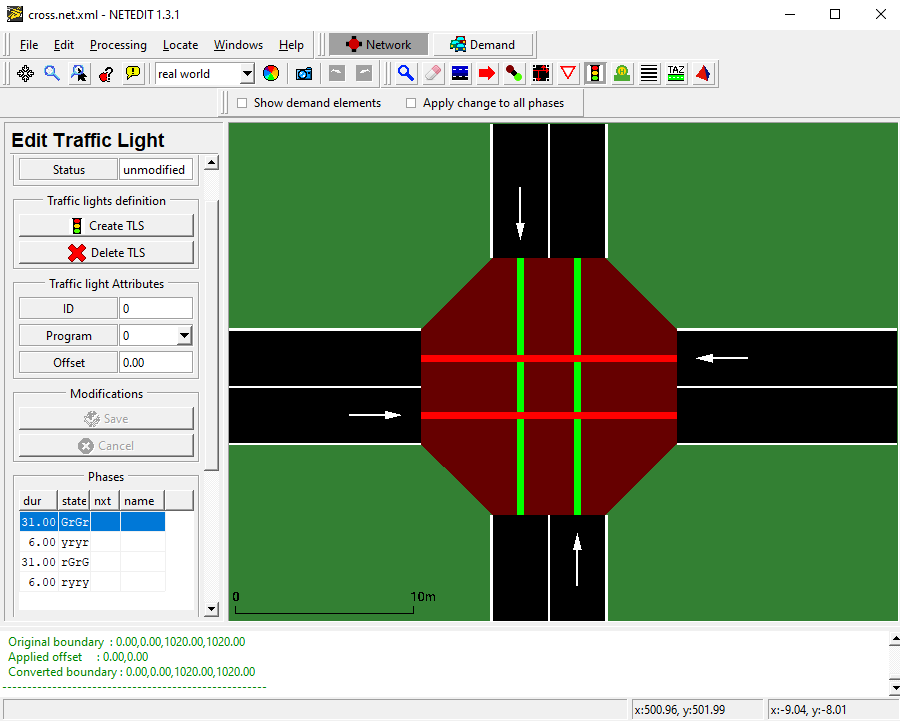
\includegraphics[width=\textwidth]{sumo/1cb8aa292f0be15b402ccd4f098f53e0.png}
    \caption{Editor gráfico NETEDIT mostrando una intersección y el menú de edición de semáforos.}
    \label{fig:netedit1}
\end{figure}

\begin{figure}[H]
    \centering
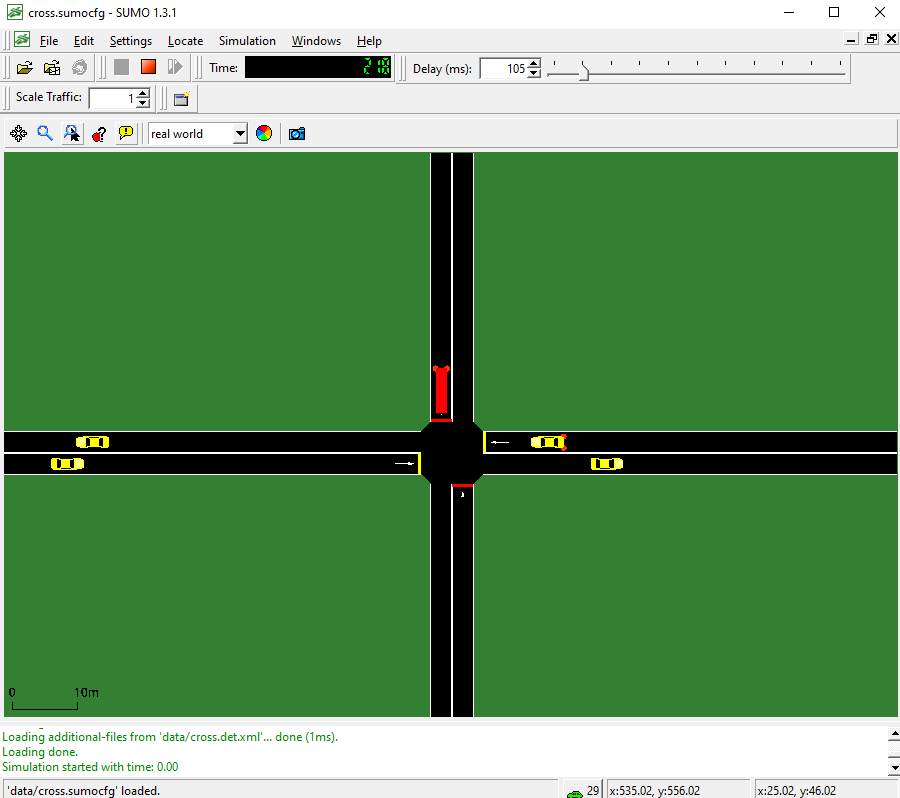
\includegraphics[width=\textwidth]{sumo/f06ad63e2235a639007f9748f2326f91.png}
    \caption{Simulando la intersección anterior de manera gráfica en SumoGui.}
    \label{fig:sumogui1}
\end{figure}

\begin{figure}[H]
    \centering
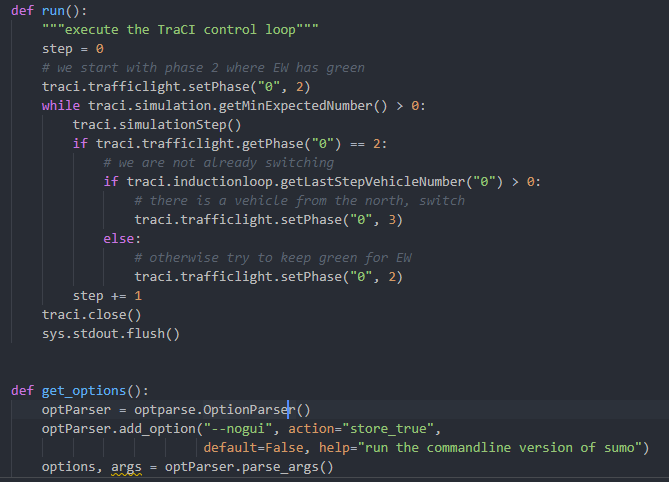
\includegraphics[width=\textwidth]{sumo/8a185a540ef5e98b250d7c70216cddfc.png}
    \caption{Controlando los semáforos desde Python con TraCI (Traffic Control Interface).}
    \label{fig:traci1}
\end{figure}

\begin{figure}[H]
    \centering
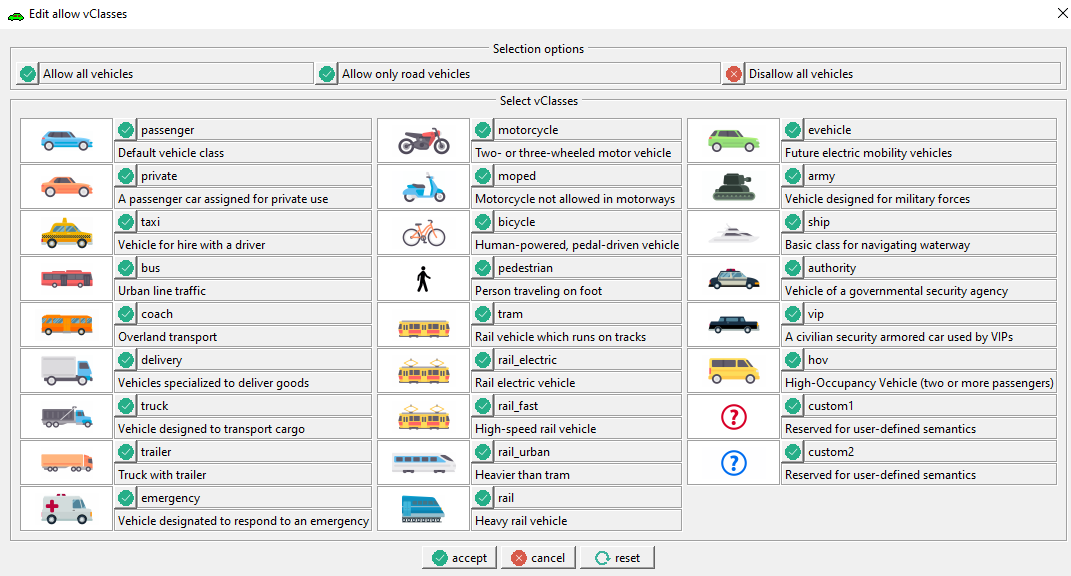
\includegraphics[width=\textwidth]{sumo/d600ef6ce1de01e90d10a436d7b6bb75.png}
    \caption{Los diversos tipos de vehículos disponibles.}
    \label{fig:sumogui2}
\end{figure}

\hypertarget{simulaciuxf3n-de-semuxe1foros}{%
\subsection{Simulación de
semáforos}\label{simulaciuxf3n-de-semuxe1foros}}

Los semáforos (llamados en el simulador TLS - \emph{Traffic Light
System}) se pueden crear de manera gráfica en NETDIT y automáticamente
generan un programa de control.

\begin{figure}[H]
    \centering
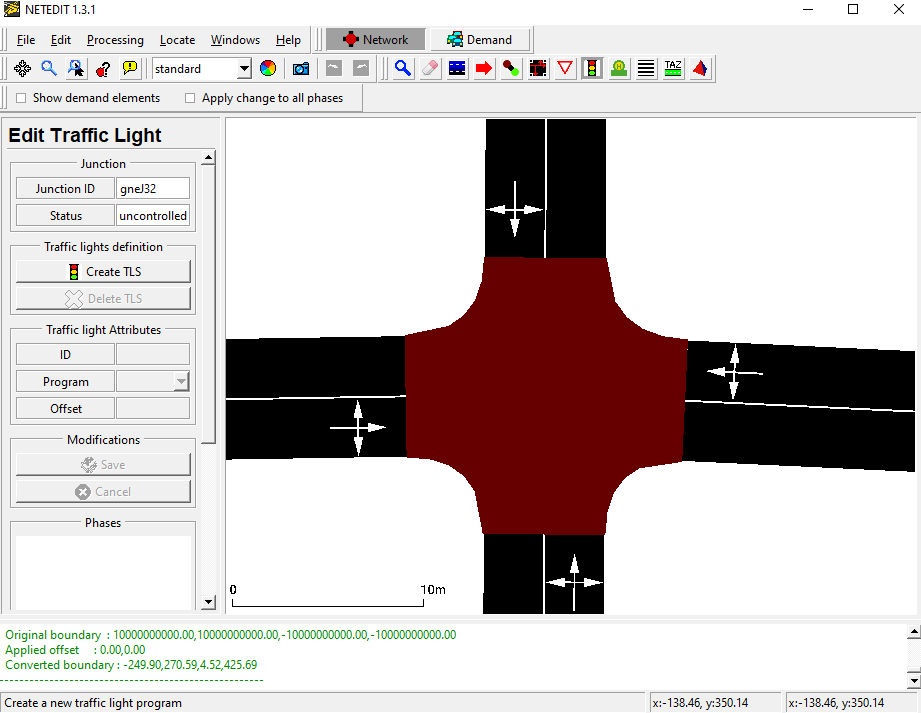
\includegraphics[width=\textwidth]{sumo/d53e12f08f94d08fd7e31f214786b43e.png}
    \caption{Creando gráficamente un programa de control de semáforo en NETDIT.}
    \label{fig:netedit2}
\end{figure}

\begin{figure}[H]
    \centering
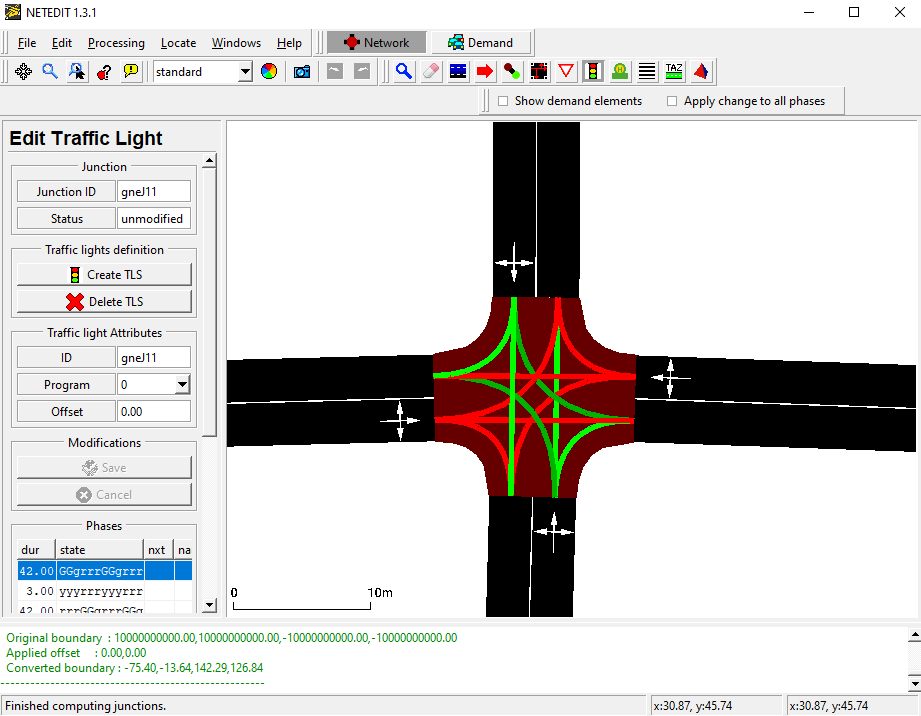
\includegraphics[width=\textwidth]{sumo/e760085ba60c72e71c15ed1d0d5ab9aa.png}
    \caption{Vista gráfica de reglas de paso de un programa de control de
    tráfico en NETEDIT.}
    \label{fig:netedit3}
\end{figure}

\hypertarget{definiciuxf3n-de-nuevos-programas-tls}{%
\subsection{Definición de nuevos programas
TLS}\label{definiciuxf3n-de-nuevos-programas-tls}}

Se puede cargar nuevas definiciones para semáforos como parte de un
archivo adicional. La definición de un programa de semáforo dentro de un
archivo adicional se ve así:

\begin{lstlisting}[language=XML]
<additional>
    <tlLogic id="semaforo_principal" type="static" programID="principal" offset="0">
        <phase duration="40" state="GrGr"/>
        <phase duration="6" state="yryr"/>
        <phase duration="40" state="rGrG"/>
        <phase duration="6" state="ryry"/>
    </tlLogic>
</additional>
\end{lstlisting}

Cada programa está compuesto de varias fases de cierta duración. En cada
una, el atributo \emph{state} define con una cadena de códigos que se
corresponden con los colores de todos los semáforos en esa fase. El
significado de los códigos principales se puede ver en la siguiente
tabla:

\begin{table}[h!]
\centering
\begin{tabular}[t]{c l m{11cm}}
    \toprule
    Código  & Color        & Descripción                                                                                         \\
    \midrule
    r       & rojo         & Luz roja: los vehículos deben detenerse.                                                            \\ 
    y       & amarillo     & Luz amarilla:los vehículos desacelerarán si están lejos de la insersección, de lo contrario pasarán.\\
    G       & verde        & Luz verde de prioridad: los vehículos pasarán.                                                      \\
    \bottomrule
\end{tabular}
\caption{}
\label{table:tab1}
\end{table}

La posiciónde cada caracter en la cadena se corresponde con las
conexiones de la insercción controlada empezando desde arriba en el
orden de las manecillas del reloj. Por ejemplo, la siguiente imagen se
corresponde con la cadena \texttt{state\ =\ "GrGr"}.

\begin{figure}[H]
    \centering
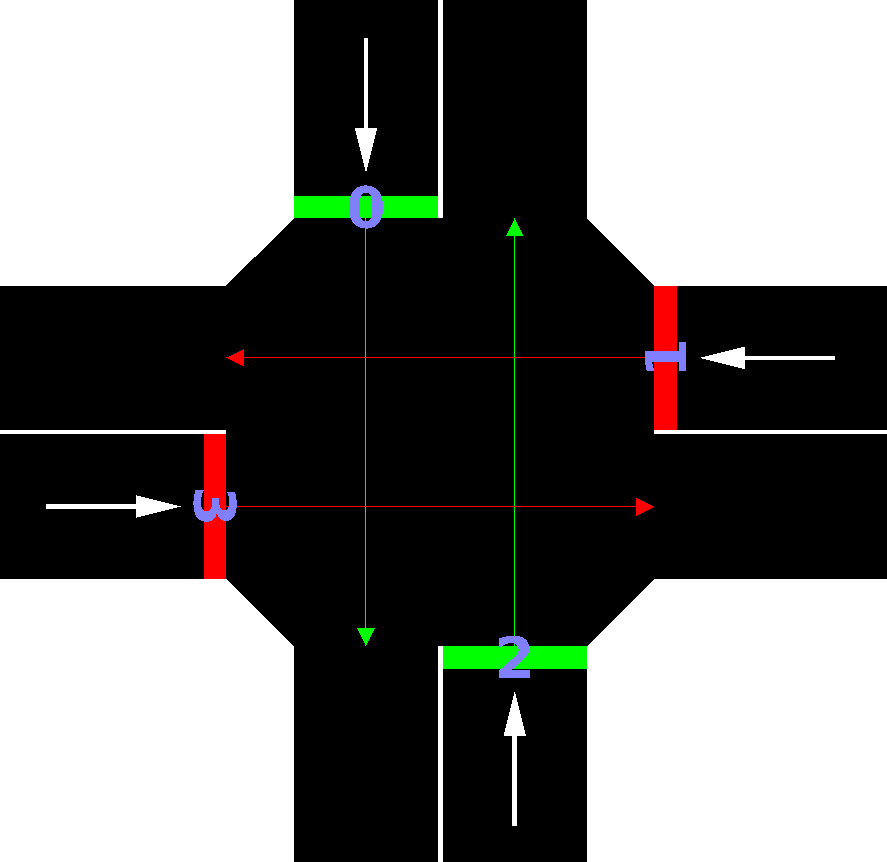
\includegraphics[width=\textwidth]{sumo/tls_light_order.png}
    \caption{Correspondencia de cadenas de códigos a colores de semáforo.}
    \label{fig:netedit4}
\end{figure}

\hypertarget{control-de-los-semuxe1foros-con-python}{%
\subsection{Control de los semáforos con
Python}\label{control-de-los-semuxe1foros-con-python}}

Más importante aún, también es posible controlar los estados de los
semáforos programáticamente a través de una interfaz incluida en el
paquete de instalación llamada TraCI.

TraCI es la abreviatura de
``~\textbf{Tra}fic~\textbf{C}ontrol~\textbf{I}nterface''.~Al dar acceso
a una simulación de tráfico en ejecución, permite recuperar valores de
objetos simulados y manipular su comportamiento ``en línea''.

TraCI utiliza una arquitectura cliente / servidor basada en TCP para
proporcionar acceso a SUMO. De este modo, SUMO actúa como servidor y el
código Python con TraCI como cliente.

A continuación, se muestra el código de ejemplo que controla la lógica
del semáforo para que se controle de la siguiente manera:

\begin{figure}[H]
    \centering
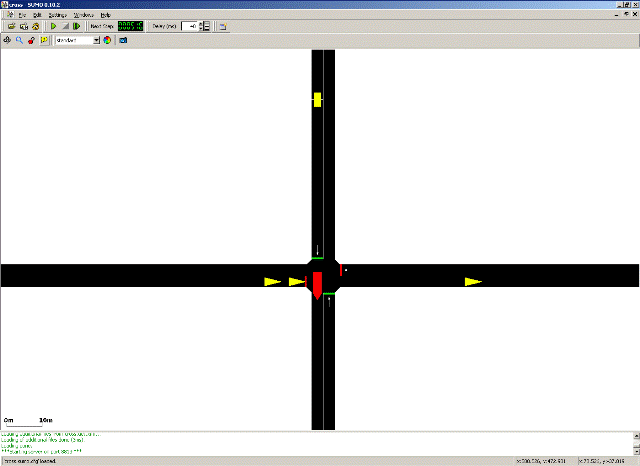
\includegraphics[width=\textwidth]{sumo/3a9d001be95c93c93c1c13ed9aeb7b26.png}
    \caption{Ejemplo de intersección de cuatro vías.}
    \label{fig:sumogui3}
\end{figure}

El ejemplo muestra una simple intersección de cuatro vías. Hay tráfico
normal en el eje horizontal y vehículos importantes (ambulancias,
patrullas, camiones de bomberos, etc.) en el eje vertical de norte a
sur. En la vía que viene desde el norte hay un detector para reconocer a
los vehículos que van entrando. Mientras que ningún vehículo ingresa
desde el norte, siempre damos color verde en el eje horizontal, pero
cuando un vehículo ingresa al circuito del detector, cambiamos la señal
de inmediato para que el vehículo pueda cruzar la intersección sin
detenerse.

\begin{lstlisting}[language=Python]
step = 0
traci.trafficlight.setPhase("0", 2)
while traci.simulation.getMinExpectedNumber() > 0:
    traci.simulationStep()
    if traci.trafficlight.getPhase("0") == 2:
        if traci.inductionloop.getLastStepVehicleNumber("0") > 0:
            traci.trafficlight.setPhase("0", 3)
        else:
            traci.trafficlight.setPhase("0", 2)
    step += 1
traci.close()
\end{lstlisting}

\hypertarget{creaciuxf3n-de-simulaciuxf3n}{%
\section{Creación de simulación}\label{creaciuxf3n-de-simulaciuxf3n}}

Para probar y desarrollar a detalle la arquitectura se usará el
simulador de tráfico urbano SUMO, que incluye prácticamente todas las
herramientas necesarias.

\hypertarget{red-de-carreteras}{%
\subsection{Red de carreteras}\label{red-de-carreteras}}

El primer paso para crear una simulación en SUMO consiste en crear una
red de carreteras. Dichas redes deben estar definidas en un archivo con
extensión .net.xml que puede ser creado de múltiples maneras. Una de
ellas es utilizando la aplicación netconvert (incluida en la instalación
base), que se encarga de importar redes de carreteras de diferentes
fuentes que pueden ser usadas por otras herramientas del paquete
incluído en SUMO. También es posible utilizar la aplicación gráfica
netedit para editar una red previamente creada con netconvert o incluso
crear una desde cero con la misma aplicación.

El método usado para crear la red de carreteras que utilizará la
sumulación es una combinación de los dos anteriores. Se creó la red de
tráfico usando un script llamado
\href{https://sumo.dlr.de/docs/Tutorials/OSMWebWizard.html}{osmWebWizard},
que permite seleccionar un área geográfica real desde OpenStreetMaps y
convertirla en el red con extensión .net.xml que utiliza SUMO.

Para motivos de prueba, se usó una intersección de Mérida conocida, para
poder simular flujos a partir de lugares familiares, y en dado caso de
ser necesario recolectar datos reales. La intersección en cuestión está
ubicada en el sur de la ciudad, donde Circuito Colonias se cruza con la
calle 50.

Para corroborar que los datos generados por el script sean certeros, se
comparó la generación de la intersección con imágenes reales de Google
Maps, y hubo que ajustar el ancho del carril que corresponde a la calle
50 de uno a dos carriles (realmente tiene como 4, pero siempre hay
coches estacionados a ambos costados, al final se pueden aprovechar solo
2). Desconozco si las calles adyacentes tienen el ancho correcto, pero
considero que solo ésta afectan al objetivo de la simulación.

Los datos recuperados por osmWebWizard, a excepción al numero de
carriles de la calle 50, fueron bastante certeros, y la intersección de
interés tiene correctamente los derechos de paso del semáforo.

Una vez montada la simulación, fue necesario prepararla para manipularse
programáticamente, por lo que el semáforo a controlar se renombró a
\emph{semaforo\_circuito\_colonias} y se modificó el comportamiento de
los semáforos para que sean estáticos y solo cambien cuando se les
indique manualmente usando código.

\hypertarget{modelado-de-la-arquitectura}{%
\subsection{Modelado de la
arquitectura}\label{modelado-de-la-arquitectura}}

Con la red de tráfico lista, el objetivo es programar la arquitectura
previamente propuesta en Python, y para ello se utilizará una interfaz
para manipular la simulación en tiempo real llamada TraCI. Dicha
interfaz ya viene incluído en la instalación por defecto de SUMO.

Los primeros módulos de la arquitectura a programar son el
\emph{Observador de eventos} y el \emph{Registrador de eventos}, y para
ello se modelaron las propiedades de una intersección en clases que se
relacionan entre si.

La más básica es Edge, que es lo equivalente a una calle y contiene sus
propiedades asociadas:

\begin{itemize}
\item
  conection\_uses\_from: relaciona el Edge con una Conection.
\item
  conection\_uses\_to: relaciona el Edge con una Conection.
\item
  name: nombre o apodo para la calle.
\item
  num\_lanes: numero de carriles.
\item
  is\_traffic\_input: indica si el trafico entra por esta calle.
\item
  associated\_detector\_name: nombre del detector de trafico asociado a
  esta calle.
\item
  street\_name: nombre real de la calle.
\item
  aprox\_length: largo aproximado de la calle.
\item
  aprox\_total\_width: ancho aproximado de la calle completa que incluye
  a todos los carriles.
\end{itemize}

Las calles están conectadas entre si, y esta relación se representa a
través de la clase Conection, que indica una conexión simple entre Edges
(calles):

\begin{itemize}
\item
  intersection: relaciona que una Intersection puede tener varias
  Conections.
\item
  from\_edge: desde que calle viene el trafico.
\item
  to\_edge: hacia que calle viene el trafico.
\end{itemize}

Las calles se agrupan en intersecciones que tienen conexiones entre
ellas y posiblemente un semáforo. Esto se representa en la clase
Intersection:

\begin{itemize}
\item
  name: nombre o apodo para la intersección.
\item
  associated\_traffic\_light\_name: el nombre del semáforo asociado a la
  intersección.
\item
  conections: lista de todas las conexiones entre calles.
\end{itemize}

Siguiendo la arquitectura, los datos de cada intersección y del estado
de la simulación deben almacenarse en algún lugar para posteriormente
realizar un reporte que se guardará para su análisis. Se escogió medio
de almacenamiento temporal una base de datos en sqlite, y se utilizó la
librería Pony ORM para convertir el modelado en clases a tablas de una
base de datos.

Actualmente se está trabajando en la implementación del framework Flow,
que permite manipular conectar fácilmente SUMO con librerías de
Reinforcement Learning, así como incluye métodos para generar tráfico de
manera más realista.

\clearpage % Nueva página

% \clearpage
% \newpage
\thispagestyle{empty}
\vspace*{\fill}
\begingroup
\centering
\begin{flushright}{\fontsize{50}{60}\selectfont CAPÍTULO 3}\end{flushright}
\vspace{10 mm}
\begin{flushright}{\fontsize{30}{40}\selectfont METODOLOGÍA }\end{flushright}
\endgroup
\vspace*{\fill}
\newpage
% 
\chapter{Desarrollo} % con la palabra capitulo
\graphicspath{{./../imagenes/}}
\linespread{1.3}
\hypertarget{propuesta-de-arquitectura}{%
\section{Propuesta de Arquitectura}\label{propuesta-de-arquitectura}}

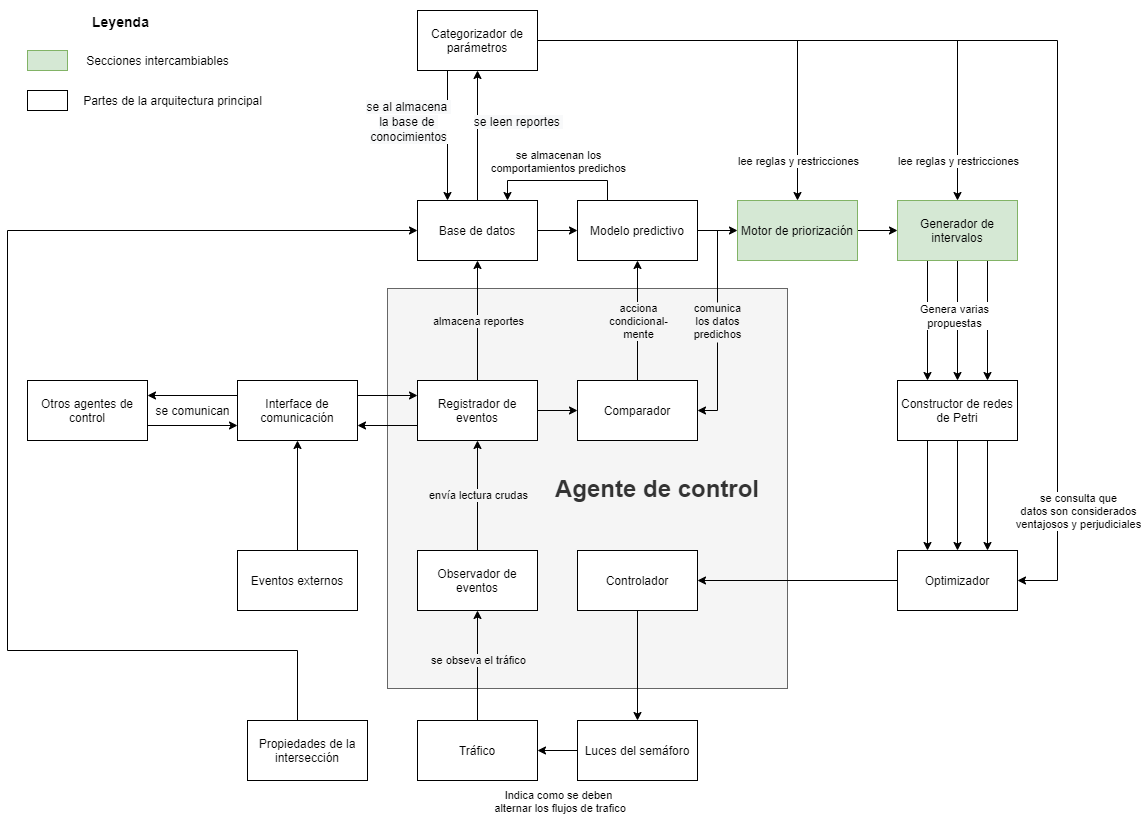
\includegraphics[width=\textwidth]{arquitectura.png} Fig. 1:
Arquitectura de un agente de control.

\hypertarget{truxe1fico}{%
\subsection{Tráfico}\label{truxe1fico}}

Los vehículos que se mueven en los carriles de la intersección y cruzan
de un carril a otro en nodos llamados intersecciones. Sobre las
intersecciónes puede haber ubicados semáforos.

\hypertarget{propiedades-de-la-intersecciuxf3n}{%
\subsection{Propiedades de la
intersección}\label{propiedades-de-la-intersecciuxf3n}}

Son las propiedades intrínsecas de la intersección que no suelen cambiar
con el paso del tiempo:

\begin{itemize}
\tightlist
\item
  Número de calles.
\item
  Carriles en cada calle.
\item
  Extensión aproximada de cada carril.
\item
  Estructura de la intersección: todas las posibles conexiones entre
  carriles.
\item
  Derechos y prioridades de paso.
\item
  Disposición de las luces del semáforo (cuántas hay y a que
  intersección apuntan).
\item
  Existencia de cruces y puentes peatonales, y si tienen algún botón que
  permita detener el tráfico.
\end{itemize}

\hypertarget{observador-de-eventos}{%
\subsection{Observador de eventos}\label{observador-de-eventos}}

Su única tarea es ser el sentido de la vista del agente de control.
Tiene funciones para observar eventos de interés que suceden con
regularidad en el mundo real en un momento dado y sus propiedades, tales
como:

\begin{itemize}
\tightlist
\item
  El paso de los vehículos, con propiedades como:

  \begin{itemize}
  \tightlist
  \item
    Ruta que toma (pueden seguir derecho o girar en algún sentido).
  \item
    Velocidad promedio aproximada.
  \item
    Cuanto tiempo permanece detenido.
  \item
    Aceleración aproximada.
  \end{itemize}
\item
  Cambios de luces (en que carril y a que color cambió).
\end{itemize}

Y también notifica eventos emergentes y sus propiedades, como:

\begin{itemize}
\tightlist
\item
  Aparición de un vehículos de prioridad (de que tipo y en que carril).
\item
  Un accidente (que carril obstruye).
\end{itemize}

Todo lo observado lo comunica al \emph{Registrador de eventos} indicando
el tiempo exacto en el que sucedió (\emph{timestamp}).

\hypertarget{registrador-de-eventos}{%
\subsection{Registrador de eventos}\label{registrador-de-eventos}}

Es el encargado de guardar un caché de los datos crudos enviados por el
\emph{Observador de eventos} e interpretarlos, para cada hora generar
reportes con datos derivados que se almacenan en la base de datos. El
reporte generado agrupa los datos por ciclo de semáforo, siendo éstos
los siguientes:

\begin{itemize}
\tightlist
\item
  Flujo por carril, es decir, el número de vehículos que pasan por cada
  carril cada determinado tiempo.
\item
  Tiempo de espera promedio por carril.
\item
  Densidad de cada carril.
\item
  Cola más larga en la señal roja.
\item
  Número de vehículos que pasan en señal verde.
\item
  Tiempo ocioso de la señal verde.
\item
  Cola más larga próxima fase.
\item
  Tiempo de cambio de la cola más larga en señal roja.
\end{itemize}

También recibe datos al exterior a través de la \emph{Interfaz de
comunicación}, que se almacenan selectivamente en la base de datos.

\hypertarget{interfaz-de-comunicaciuxf3n}{%
\subsection{Interfaz de
comunicación}\label{interfaz-de-comunicaciuxf3n}}

Permite enviar y recibir reportes de otros agentes de control, así como
notificaciones de eventos externos que pueden alterar el tráfico, como:

\begin{itemize}
\tightlist
\item
  Alertas de desastre natural.
\item
  Eventos públicos y días festivos.
\item
  Manifestaciones.
\end{itemize}

\hypertarget{comparador}{%
\subsection{Comparador}\label{comparador}}

Se encarga de comparar constantemente el comportamiento de los eventos
registrados con el comportamiento predicho. Cuando estos difieren de
manera significativa, el comparador solicita al \emph{Modelo predictivo}
que genere una nueva predicción. También se encarga de solicitar nuevas
predicciones cada que un evento externo lo solicite.

\hypertarget{modelo-predictivo}{%
\subsection{Modelo predictivo}\label{modelo-predictivo}}

Se alimenta del histórico de reportes generados por el \emph{Registrador
de eventos} que obtiene de la base de datos para predecir del
comportamiento de una intersección durante la siguiente hora. Los datos
que genera son los mismos que figuran el los reportes creados por el
\emph{Registrador de eventos}. También hace predicciones bajo demanda
cuando el \emph{Comparador} lo solicita.

\textbf{(Incluir aquí gráfica que represente el rango de tiempo en el
que son válidas las predicciones, la estimación de pérdida de tiempo
efectivo por el tiempo de generación, etc.)}

Ya que el proceso de hacer una predicción y su posterior optimización es
un proceso intensivo, las peticiones para nuevas predicciones suceden
cada hora, pero de manera escalonada. Por ejemplo: si existen 4 agentes
de control, uno iniciará una petición de predicción a las 2:00 p.m.,
mientras que otra los hará a las 2:15 p.m., otro a las 2:30, y así
sucesivamente, de tal manera que el tiempo entre cada hora se se reparta
lo más igualitariamente posible. De la mano con estas peticiones
escalonadas, las peticiones se realizarán de manera asíncrona usando
hilos de procesamiento para lograr paralelizar el procesamiento de
varias intersecciones a la vez de ser necesario. De esta manera, se
aprovecha también el sistema de encolamiento de hilos nativo de los
sistemas operativos, que resulta particularmente útil para no atrasar
las predicciones programadas por las realizadas bajo demanda.

\hypertarget{categorizador-de-paruxe1metros}{%
\subsection{Categorizador de
parámetros}\label{categorizador-de-paruxe1metros}}

Se encarga de categorizar la influencia de los parámetro predichos entre
sí mismos y como finalmente influyen sobre el comportamiento global del
tráfico, para así obtener conclusiones en forma de restricciones y
reglas aplicadas para al temporizado de los ciclos del semáforo.
Categoriza intervalos de tiempo que presentan una serie de condiciones a
términos abstractos, como: ``hora pico'', ``hora sin actividad'' o
``tráfico esporádico'', para así poder usar esas categorías como
condiciones para las reglas y restricciones vistas anteriormente.
Categoriza como ventajoso o perjudicial el incremento o decremento de un
parámetro respecto a parámetros que se busquen incrementar o decrementar
(como el tiempo de espera, la generación de colas, etc). De ser
necesario, infiere una función de como su variación afecta a estos
parámetros.

Ejemplo verbal: si se hacen ciclos en verde un un carril \textbf{mayores
a} 45 segundos durante \textbf{horas pico}, se genera una \textbf{cola
de espera perjudicial a la fluidez} del carril perpendicular, entonces
se infiere una regla que impida que se rebase ese tiempo de ciclo dadas
esas condiciones, y en caso de que se tenga que se rebase, se tenga la
función que indica que tanto perjudica ese aumento para calcular los
tiempos de ciclo que produzcan el mejor costo-beneficio (pues se tienen
que tomar en cuenta el resto de los parámetros).

Este módulo analiza constantemente los reportes almacenados en la base
de datos para realizar el proceso mencionado anteriormente y todo lo
inferido se guarda de manera centralizada como una base de conocimientos
central como registros en la base de datos.

Este módulo se inspiro en la llamada \emph{Colección de hechos} usada en
\textcite{JoelTrejo2006}.

\begin{quote}
La colección de hechos alberga los datos correspondientes a la
aplicación de determinada estrategia de control cuando se presentan
ciertas condiciones en el tráfico observado. La colección de hechos
puede desempeñar el papel de memoria auxiliar en la cual se registran
los razonamientos llevados a cabo. \textcite[p. 47]{JoelTrejo2006}
\end{quote}

\hypertarget{motor-de-priorizaciuxf3n}{%
\subsection{Motor de priorización}\label{motor-de-priorizaciuxf3n}}

Se encarga de asignar un valor numérico a cada carril, que indica su
prioridad. Entre mayor el número, mayor la prioridad. Este número de
genera usando como base la demanda predicha, aunque también es posible
usar restricciones y reglas definidas por el \emph{Categorizador de
parámetros}.

\hypertarget{generador-de-intervalos}{%
\subsection{Generador de intervalos}\label{generador-de-intervalos}}

Usa los valores generados por el \emph{Motor de priorización} para
generar una proporción de la duración de cada fase del semáforo en la
duración total del ciclo. Posteriormente usa como base las reglas y
restricciones generados por el \emph{Categorizador de parámetros} para
generar varias propuestas de la duración total del ciclo de fases de
luces. Se obtiene como salida varios juegos de propuestas de duraciones
de fases que pueden haber tomado en cuenta diferentes reglas.

\hypertarget{constructor-de-redes-de-petri}{%
\subsection{Constructor de redes de
Petri}\label{constructor-de-redes-de-petri}}

A partir de las propuestas de intervalos generadas por el
\emph{Generador de intervalos}, se encarga de construir una red de Petri
temporizada para cada una de ellas.

\hypertarget{optimizador}{%
\subsection{Optimizador}\label{optimizador}}

Recibe múltiples propuestas de redes de Petri y a través de algoritmos
genéticos, cruza los genes de las diferentes propuestas (que tomaron en
cuenta diferente reglas para construirse) buscando maximizar los
parámetros considerados como ventajosos (como el flujo) y minimizar los
considerados como perjudiciales (como las cosas y los tiempos de
espera). La información de cuáles son estos parámetros se obtiene del
\emph{Categorizador de parámetros}. Al final da como salida una red de
Petri optimizada.

\hypertarget{controlador}{%
\subsection{Controlador}\label{controlador}}

Tiene las funciones para necesarias para leer la red de Petri
temporizada que recibe y controlar los cambios de luces según lo indique
la red.

\hypertarget{luces-de-semuxe1foro}{%
\subsection{Luces de semáforo}\label{luces-de-semuxe1foro}}

Son la manera en la que se plasman los intervalos de luces generados y
son lo que físicamente indica a los conductores cuando deben circular o
detenerse.

\clearpage % Nueva página

% \clearpage
% \newpage
\thispagestyle{empty}
\vspace*{\fill}
\begingroup
\centering
\begin{flushright}{\fontsize{50}{60}\selectfont CAPÍTULO 4}\end{flushright}
\vspace{10 mm}
\begin{flushright}{\fontsize{30}{40}\selectfont RESULTADOS }\end{flushright}
\endgroup
\vspace*{\fill}
\newpage
% \chapter{Resultados}\label{cap4} % con la palabra capitulo
\graphicspath{{./graficas}}
%\addcontentsline{toc}{chapter}{Capítulo 2: Marco Teórico} % si queremos que aparezca en el Í­ndice
%\markboth{Capítulo 2: Marco Teórico}{Capítulo 2: Marco Teórico} % encabezado
\linespread{1.3}
En la Figura \ref{fig:graf} se muestra un ejemplo de una grafica añadida en formado .pdf (puede utilizarse formato .jpg, .png o directamente desde software graficador en formato .tex)
\begin{figure}[hbtp]
\centering
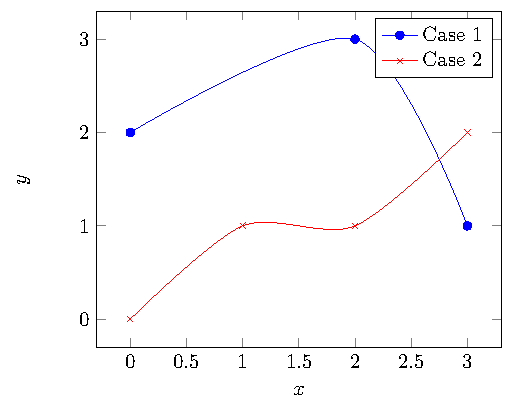
\includegraphics[scale=1]{/pg.pdf}
\caption{ejemplo de gráfica.}
\label{fig:graf}
\end{figure}
\clearpage%
\clearpage
\newpage
\thispagestyle{empty}
\vspace*{\fill}
\begingroup
\centering
\begin{flushright}{\fontsize{30}{40}\selectfont CONCLUSIONES}\end{flushright}
\endgroup
\vspace*{\fill}
\newpage
\chapter*{Conclusiones} % si no queremos que añada la palabra "Capitulo"
\addcontentsline{toc}{chapter}{Conclusiones} % si queremos que aparezca en el Í­ndice
\markboth{CONCLUSIONES}{CONCLUSIONES} % encabezado

\linespread{1.3}

\clearpage % Nueva página
\clearpage
%-----------------------------------------------------------------------------------------------------------------
%         B I B L I O G R A F I A   Y   A P E N D I C E S
%-----------------------------------------------------------------------------------------------------------------
\bibliographystyle{IEEEtran-spanish} % Tipo de bibliografía
\bibliography{bibliografia} % Incluye la bibliografía
\clearpage 
\newpage
\thispagestyle{empty}
\vspace*{\fill}
\begingroup
\centering
\begin{flushright}{\fontsize{30}{40}\selectfont APÉNDICE}\end{flushright}
\endgroup
\vspace*{\fill}
\newpage
\chapter*{Apéndice A} % si no queremos que añada la palabra "Capitulo"
\addcontentsline{toc}{chapter}{Apéndice A} % si queremos que aparezca en el Í­ndice
\markboth{Ap\'endice A}{Ap\'endice A} % encabezado

\linespread{1.3}

\noindent \textbf{\large{Software Utilizado}}
\ \newline
\par

En el presente trabajo se usaron los siguientes programas.

\begin{itemize}
	\item Programa 1
	\item Programa 2
	\item Programa 3
	\item Programa 4
	
\end{itemize}

Este trabajo ha sido escrito completamente en  \LaTeX usando el editor de texto Visual Studio Code con la extensión LaTeX Workshop desde archivos fuente en Markdown convertidos con Pandoc.
\clearpage % Nueva página




% \begin{versionhistory} 
% \begin{center}
%  \textbf{\docTitle}\\
%  \textbf{\vhListAllAuthors}\\
%  \textbf{Version} \vhCurrentVersion\ \\
% Fecha \vhCurrentDate
% \end{center} 
%  \vhEntry{1.0}{03.01.19}{MHO}{creado}
%  \vhEntry{1.1}{03.01.19}{JARB|CABH}{correcci\'{o}n}
%  \vhEntry{1.2}{05.01.19}{JARB|CABH}{revisado después de correcci\'{o}n}
% \end{versionhistory}
\clearpage % Incluye el apéndice
%-----------------------------------------------------------------------
\end{document}%